\documentclass[aspectratio=169,11pt]{beamer}

\usetheme{Madrid}
\usecolortheme{default}
\setbeamertemplate{navigation symbols}{}
\setbeamertemplate{footline}[frame number]

\usepackage[T1]{fontenc}
\usepackage[utf8]{inputenc}
\usepackage{lmodern}
\usepackage{amsmath}
\usepackage{booktabs}
\usepackage{tabularx}
\usepackage{tikz}
\usepackage{listings}
\usepackage{xcolor}
\usetikzlibrary{positioning}

\definecolor{sdmblue}{RGB}{27, 74, 125}
\definecolor{sdmteal}{RGB}{0, 130, 127}
\definecolor{sdmorange}{RGB}{222, 123, 35}
\definecolor{sdmlight}{RGB}{244, 247, 250}
\definecolor{codebg}{RGB}{247, 248, 250}

\setbeamercolor{structure}{fg=sdmblue}
\setbeamercolor{palette primary}{bg=sdmblue, fg=white}
\setbeamercolor{palette secondary}{bg=sdmteal, fg=white}
\setbeamercolor{palette tertiary}{bg=sdmblue, fg=white}
\setbeamercolor{title}{fg=sdmblue}
\setbeamercolor{frametitle}{bg=sdmblue!8, fg=sdmblue}
\setbeamercolor{block title}{bg=sdmblue, fg=white}
\setbeamercolor{block body}{bg=sdmlight, fg=black}
\setbeamercolor{alerted text}{fg=sdmorange}

\lstset{
  basicstyle=\ttfamily\scriptsize,
  backgroundcolor=\color{codebg},
  frame=single,
  rulecolor=\color{sdmblue!30},
  columns=fullflexible,
  keepspaces=true,
  showstringspaces=false,
  breaklines=true
}

\title{SDM-5031-2026-Spring Project}
\subtitle{Using Deep Reinforcement Learning to Solve TSP}
\author{Course Project Briefing}
\date{Spring 2026}

\begin{document}

\begin{frame}[plain]
  \vspace{0.5cm}
  {\usebeamerfont{title}\color{sdmblue}\LARGE\textbf{SDM-5031-2026-Spring Project}\par}
  \vspace{0.2cm}
  {\usebeamerfont{subtitle}\Large Using Deep Reinforcement Learning to Solve TSP\par}
  \vspace{0.6cm}

  \begin{columns}[T,totalwidth=\textwidth]
    \begin{column}{0.60\textwidth}
      \begin{block}{What students should leave with}
        \begin{itemize}
          \item A stronger TSP solver than the provided baseline
          \item A clean experimental pipeline on the public validation set
          \item A report and presentation that explain method novelty clearly
        \end{itemize}
      \end{block}
    \end{column}
    \begin{column}{0.38\textwidth}
      \begin{alertblock}{Critical reminder}
        Public validation set $\neq$ final hidden test set

        Official performance metric: \texttt{avg\_aug\_gap}
      \end{alertblock}
    \end{column}
  \end{columns}

  \vfill
\end{frame}

\begin{frame}{Project at a Glance}
  \begin{columns}[T,totalwidth=\textwidth]
    \begin{column}{0.54\textwidth}
      \begin{block}{Core task}
        Build a DRL-based method that solves TSP better than the bundled POMO baseline.
      \end{block}
      \begin{itemize}
        \item Starter code already includes training and evaluation scripts
        \item Use the public validation set to iterate and compare \texttt{avg\_aug\_gap}
        \item Final grading will use the same interface on a hidden test set
      \end{itemize}
    \end{column}
    \begin{column}{0.42\textwidth}
      \centering
      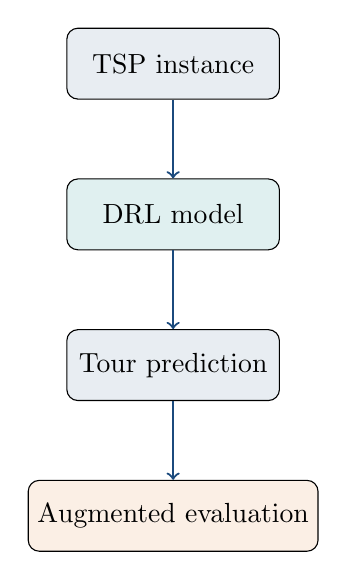
\begin{tikzpicture}[node distance=1.0cm, every node/.style={align=center}]
        \node[draw, rounded corners, fill=sdmblue!10, minimum width=2.7cm, minimum height=0.9cm] (a) {TSP instance};
        \node[draw, rounded corners, fill=sdmteal!12, minimum width=2.7cm, minimum height=0.9cm, below=of a] (b) {DRL model};
        \node[draw, rounded corners, fill=sdmblue!10, minimum width=2.7cm, minimum height=0.9cm, below=of b] (c) {Tour prediction};
        \node[draw, rounded corners, fill=sdmorange!12, minimum width=2.7cm, minimum height=0.9cm, below=of c] (d) {Augmented evaluation};
        \draw[->, thick, sdmblue] (a) -- (b);
        \draw[->, thick, sdmblue] (b) -- (c);
        \draw[->, thick, sdmblue] (c) -- (d);
      \end{tikzpicture}
    \end{column}
  \end{columns}
\end{frame}

\begin{frame}[fragile]{What You Are Given}
  \begin{columns}[T,totalwidth=\textwidth]
    \begin{column}{0.48\textwidth}
      \begin{block}{Starter repository}
\begin{lstlisting}
TSP/POMO/train.py
TSP/POMO/test.py
TSP/POMO/TSPTester_LIB.py
TSP/data/val/
TSP/POMO/result/
\end{lstlisting}
      \end{block}
    \end{column}
    \begin{column}{0.48\textwidth}
      \begin{block}{Bundled assets}
        \begin{itemize}
          \item Validation split: \texttt{TSP/data/val}
          \item Baseline: bundled POMO checkpoint at epoch 3000
          \item Evaluation entrypoint: \texttt{TSP/POMO/test.py}
        \end{itemize}
      \end{block}
      \begin{alertblock}{Important}
        The public validation set is for development only. Final acceptance will use a separate hidden test set.
      \end{alertblock}
    \end{column}
  \end{columns}
\end{frame}

\begin{frame}{How the Project Will Be Assessed}
  \begin{block}{Project scoring items}
    \begin{tabularx}{\textwidth}{>{\raggedright\arraybackslash}p{1.6cm} X}
      \toprule
      Weight & What it means \\
      \midrule
      20\% & Performance on the provided validation set, including outperforming the baseline on at least 70\% of the instances \\
      10\% & Average rank of experimental results among all students \\
      10\% & Method novelty, supported by a paper-like report and an in-class presentation \\
      \bottomrule
    \end{tabularx}
  \end{block}

  \vspace{0.3cm}
  \begin{alertblock}{Primary metric}
    Use \texttt{avg\_aug\_gap} as the headline number.

    \texttt{avg\_no\_aug\_gap} is diagnostic only and will not be treated as the official performance metric.
  \end{alertblock}
\end{frame}

\begin{frame}{Data Policy and Evaluation}
  \begin{columns}[T,totalwidth=\textwidth]
    \begin{column}{0.48\textwidth}
      \begin{block}{Available vs. hidden data}
        \begin{itemize}
          \item \texttt{TSP/data/val} is for development only
          \item The final hidden test set is not released
          \item Your headline validation number should be \texttt{avg\_aug\_gap}
        \end{itemize}
      \end{block}
    \end{column}
    \begin{column}{0.48\textwidth}
      \begin{alertblock}{What is allowed}
        \begin{itemize}
          \item You may change training-data distributions or sampling strategies
          \item You may use open-source algorithms, but you must cite and explain them
          \item Do \textbf{not} search for likely hidden-test instances and train on them
        \end{itemize}
      \end{alertblock}
    \end{column}
  \end{columns}

  \vspace{0.4cm}
  \centering
  {\Large\color{sdmorange}\textbf{Improve generalization, not hidden-test memorization.}}
\end{frame}

\begin{frame}[fragile]{Standardized Submission Interface}
  \begin{block}{Course-staff evaluation command}
\begin{lstlisting}
cd TSP/POMO
python test.py \
  --data_path /hidden_test \
  --checkpoint_path /submission/checkpoint.pt \
  --use_cuda true \
  --cuda_device_num 0 \
  --augmentation_enable true \
  --aug_factor 8 \
  --detailed_log false \
  --output_json /results/eval.json
\end{lstlisting}
  \end{block}

  \begin{itemize}
    \item Please keep this CLI stable in your submission
    \item The script prints a final \texttt{SUMMARY\_JSON: \{...\}} line to stdout
    \item The JSON file can be collected automatically for batch evaluation
  \end{itemize}
\end{frame}

\begin{frame}{What Counts as a Good Improvement?}
  \begin{columns}[T,totalwidth=\textwidth]
    \begin{column}{0.48\textwidth}
      \begin{block}{Model-side ideas}
        \begin{itemize}
          \item Better encoder or attention design
          \item More stable policy learning
          \item Smarter normalization or feature engineering
        \end{itemize}
      \end{block}
      \begin{block}{Training-side ideas}
        \begin{itemize}
          \item Better curriculum or sampling
          \item Stronger initialization or fine-tuning
          \item More careful hyperparameter search
        \end{itemize}
      \end{block}
    \end{column}
    \begin{column}{0.48\textwidth}
      \begin{block}{Inference-side ideas}
        \begin{itemize}
          \item Better use of augmentation
          \item Search or reranking at test time
          \item Improved robustness across instances
        \end{itemize}
      \end{block}
      \begin{alertblock}{Novelty matters}
        A better number alone is not enough. Explain \emph{why} the method should work and show evidence that it actually does.
      \end{alertblock}
    \end{column}
  \end{columns}
\end{frame}

\begin{frame}{Recommended Workflow for Students}
  \begin{enumerate}
    \item Reproduce the baseline result on the public validation set
    \item Decide one clear improvement idea and implement it cleanly
    \item Re-evaluate with the same interface and compare \texttt{avg\_aug\_gap}
    \item Prepare a short report and a clear classroom presentation
  \end{enumerate}

  \vspace{0.4cm}
  \begin{block}{Healthy project habits}
    Keep checkpoints organized, save exact commands, and make sure your final submission still supports the standard \texttt{test.py} interface.
  \end{block}
\end{frame}

\begin{frame}{A Few RL Training Tips}
  \begin{itemize}
    \item Do not start with a full 3000-epoch run every time. Train for a small number of epochs first and inspect the convergence curve.
    \item Use early experiments to compare trends, not just final scores. A model that learns faster is often easier to improve.
    \item Validate often on the public split so you can stop bad ideas early.
    \item Change one thing at a time: architecture, sampling strategy, reward design, or test-time inference.
    \item Save exact commands and checkpoints. In RL, it is easy to lose track of which setting actually helped.
  \end{itemize}
\end{frame}

\begin{frame}{Final Deliverables}
  \begin{block}{What to submit}
    \begin{itemize}
      \item Code repository
      \item Best checkpoint
      \item Paper-like report
      \item In-class presentation
    \end{itemize}
  \end{block}

  \begin{alertblock}{Submission deadline}
    Wednesday, May 13, 2026

    Teaching week 12
  \end{alertblock}

  \vspace{0.3cm}
  \centering
  {\Large\color{sdmblue}\textbf{Clean evaluation and clear explanation matter as much as a strong idea.}}
\end{frame}

\end{document}
